%%% Local Variables:
%%% mode: latex
%%% TeX-master: "../demo3"
%%% End:

\setlength{\baselineskip}{16pt}
\chapter{附录~D}\label{appen.d}

\begin{center}
\zihao{3}
\textbf{MaaS潜在用户出行行为与态度调查问卷}
\end{center}

\providecommand{\qbox}{$\square$\,}

本附录给出第~\ref{chap.staged}章MaaS多阶段采纳意愿陈述偏好（SP）调查所采用的调查问卷。问卷由开篇引导语与四个部分构成，依次为个人及家庭信息、出行模式调查、出行意愿调查（含单次出行情景与订阅服务情景两组SP实验）与出行态度调查。除单次出行情景与订阅服务情景的属性水平随机抽取外，问卷题目保持原貌，具体内容如下。

\vspace{0.6em}
\noindent\textbf{【引导语】}

尊敬的先生/女士：

感谢您在百忙之中参与我们的问卷调查。本次问卷调查的目的是为了收集MaaS平台潜在用户的信息，来帮助梳理现阶段MaaS平台建立和运营的机遇和挑战。在问卷结果处理的过程中，您的答案将会匿名，您的个人信息会被保密。

MaaS，出行即服务，是以活跃客流和高效的公共交通系统为基础，将不同交通服务（例如公共交通、出租车等）集成到一个可访问的数字出行服务中。这项定制的服务会根据用户的旅行需求提供最合适的解决方案。MaaS随时可用，并提供综合规划、预订和付款以及路线信息，提供便捷的出行服务。

\noindent\textbf{1．您是否听说过Mobility as a Service（MaaS）？}\\
\qbox 是\quad \qbox 否

\vspace{0.6em}
\noindent\textbf{第一部分\quad 个人及家庭信息}

\noindent\textbf{2．您的性别是：}\\
\qbox 男\quad \qbox 女

\noindent\textbf{3．您的年龄是：}\\
\qbox 18岁以下\quad \qbox 18--24岁\quad \qbox 25--34岁\quad \qbox 35--44岁\quad \qbox 45--54岁\quad \qbox 55--60岁\quad \qbox 60岁以上

\noindent\textbf{4．您的最高学历（在读或毕业）是：}\\
\qbox 博士\quad \qbox 硕士\quad \qbox 本科\quad \qbox 其它

\noindent\textbf{5．您的职业是：}\\
\qbox 专业技术人员\quad \qbox 商业/服务业人员\quad \qbox 企事业单位员工/公务员\quad \qbox 军人/警察\\
\qbox 生产、运输设备操作人员\quad \qbox 学生\quad \qbox 自由职业者\quad \qbox 离退休人员\quad \qbox 其他

\noindent\textbf{6．您的个人月收入是：}\\
\qbox 3000元以下\quad \qbox 3001--4500元\quad \qbox 4501--6000元\quad \qbox 6001--8000元\\
\qbox 8001--10000元\quad \qbox 10001--15000元\quad \qbox 15001--20000元\quad \qbox 20000元以上

\noindent\textbf{7．您的家庭年收入是：}\\
\qbox 10万元以下\quad \qbox 10--20万元\quad \qbox 20--30万元\quad \qbox 30--50万元\\
\qbox 50--70万元\quad \qbox 70--100万元\quad \qbox 100万元以上

\noindent\textbf{8．您共同居住的家庭成员数量：}\\
\qbox 0人\quad \qbox 1人\quad \qbox 2人\quad \qbox $>$2人

\noindent\textbf{9．您是否拥有驾照：}\\
\qbox 是\quad \qbox 否

\noindent\textbf{10．（如果是）您是否能够熟练驾车：}\\
\qbox 是\quad \qbox 否

\noindent\textbf{11．您是否拥有小汽车：}\\
\qbox 是\quad \qbox 否

\noindent\textbf{12．（如果是）您的家庭小汽车数量：}\\
\qbox 1辆\quad \qbox 2辆\quad \qbox 3辆及以上

\noindent\textbf{13．您是否拥有自行车或电动自行车：}\\
\qbox 是\quad \qbox 否

\vspace{0.6em}
\noindent\textbf{第二部分\quad 出行模式调查}

\noindent\textbf{14．您每周的平均市内出行次数}（从起点至终点完成一次出行目的的过程为一次出行。例如从家里到工作单位为一次出行，并不是依照中间换乘交通工具的次数来计算）\textbf{：}\\
\qbox 2次以内\quad \qbox 3--6次\quad \qbox 7--10次\quad \qbox 10次以上

\noindent\textbf{15．您在工作日平均每天市内出行总距离大约为：}\\
\qbox 5公里以内\quad \qbox 5--10公里\quad \qbox 10--20公里\quad \qbox 20--40公里\quad \qbox 40--60公里\quad \qbox 60公里以上\\
{\footnotesize 备注：北京东四环到西四环约20\,km。}

\noindent\textbf{16．您在周末平均每天市内出行总距离大约为：}\\
\qbox 5公里以内\quad \qbox 5--10公里\quad \qbox 10--20公里\quad \qbox 20--40公里\quad \qbox 40--60公里\quad \qbox 60公里以上

\noindent\textbf{17．您市内出行的主要目的是（按从高到低）：}\\
\qbox 通勤（上班上学）\quad \qbox 探亲访友\quad \qbox 商务\quad \qbox 休闲娱乐

\noindent\textbf{18．您的市内出行同行人数一般为：}\\
\qbox 0（单人出行）\quad \qbox 1--2人（家人或同事结伴）\quad \qbox 3人及以上

\noindent\textbf{19．您的主要出行方式是（按从高到低）：}\\
a.\,公共交通（公交/地铁）\quad b.\,出租车/网约车\quad c.\,私人小汽车\quad d.\,共享汽车（租车）\\
e.\,私人自行车/电动自行车/代步车\quad f.\,共享单车\quad g.\,步行

\noindent\textbf{20．如果需要多种方式组合出行时，您经常采用的组合为（从高到低）：}\\
a.\,出租车/网约车+公共交通\quad b.\,公共交通+私人自行车/电动自行车\\
c.\,公共交通+共享单车\quad d.\,公共交通+步行\\
e.\,共享汽车+私人自行车/电动自行车\quad f.\,共享单车\quad g.\,步行

\noindent\textbf{21．您每月在日常出行（城市内）的花费为：}\\
\qbox 50元以内\quad \qbox 50--150元\quad \qbox 150--300元\quad \qbox 300--400元\quad \qbox 400--800元\quad \qbox 800元以上

\noindent\textbf{22．您的出行能够被报销吗，报销比例大概有多少：}\\
\qbox 0\%（完全自付）\quad \qbox 低于20\%（偶尔）\quad \qbox 20\%--50\%（部分）\quad \qbox 50\%--80\%（经常）\quad \qbox 高于80\%（几乎全涵盖）

\noindent\textbf{23．请您回忆您的上一次市内出行的过程为}（如果涉及多种交通工具，请按如下格式分段填写）\textbf{：}\\
从（具体地址）到（\rule{1.2cm}{0.4pt}），使用（\rule{1.2cm}{0.4pt}），花费约（\rule{0.8cm}{0.4pt}）元——从（\rule{1.2cm}{0.4pt}）到（\rule{1.2cm}{0.4pt}），使用（\rule{1.2cm}{0.4pt}），花费约（\rule{0.8cm}{0.4pt}）元；\\
使用的交通工具有如下选项：\\
a.\,公共交通（公交/地铁）\quad b.\,出租车或网约车\quad c.\,私人小汽车\\
d.\,共享汽车（租车）私人自行车/电动自行车/代步车\quad e.\,共享单车\quad f.\,步行

\noindent\textbf{24．在市内出行中，若您使用MaaS，您的目的可能是（按顺序）：}\\
a.\,通勤\quad b.\,探亲访友\quad c.\,休闲娱乐\quad d.\,商务

\vspace{0.6em}
\noindent\textbf{第三部分\quad 出行意愿调查}

本部分请您根据最符合您情况的进行作答。本部分的调查分为两个场景，分别为单次出行情景和订阅服务情景。在单次出行情景中，在确定的出行起点和终点，我们列出了当前可选择几种交通方式以及他们的属性，并根据现有出行方案组合给出相应的打包服务（即MaaS方案）及服务的相关信息，请您根据您的情况选择最愿意采取的出行方案。

\vspace{0.3em}
\noindent\textbf{3.1\quad 单次出行（即走即付）情景示例}

总设置40个场景，分8组，每人回答5道题对应不同的场景（出行距离）。其中一个场景如下所示：

\par\medskip
\begin{center}
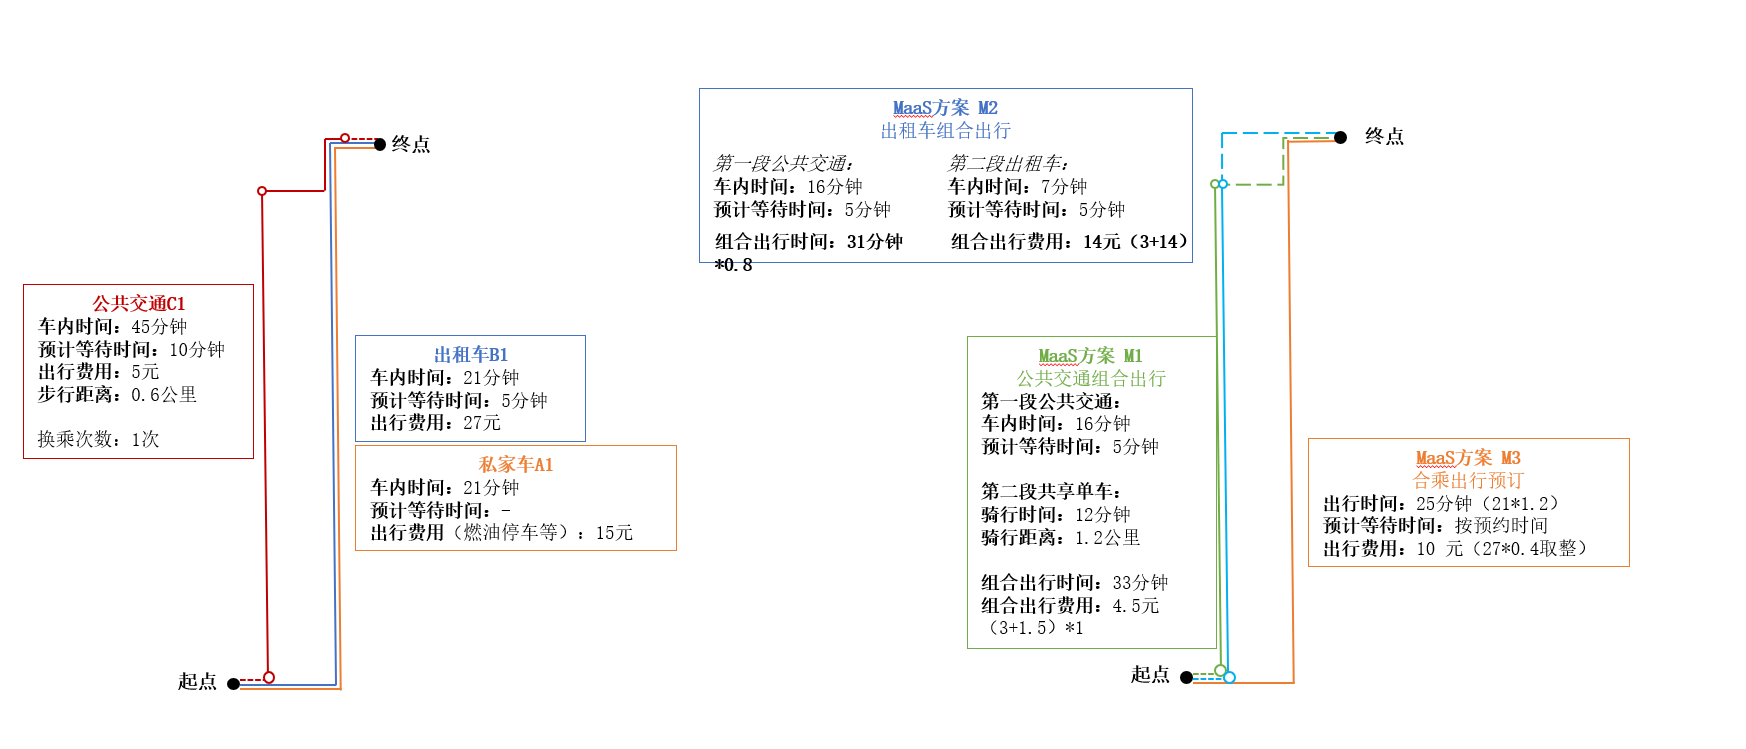
\includegraphics[width=\textwidth]{figures/appendixC/sp_single_example.png}
\end{center}
\par\medskip

如果本次出行是休闲娱乐出行，出发时间为工作日的8:00--10:00之间，今日尾号限号为：0、5（随机）。

\noindent\textbf{25．在未提供MaaS服务情况下，您会选择的出行方案是：}\\
\qbox 私家车（无车、限号请忽略）\quad \qbox 出租车/网约车\quad \qbox 公共交通

\noindent\textbf{26．如果提供了上述几种MaaS方案，您会选择的出行方案是，可以仍然保持原方案：}\\
\qbox 私家车（无车、限号请忽略）\quad \qbox 出租车/网约车\quad \qbox 公共交通\\
\qbox M1-公共交通组合出行方案\quad \qbox M2-出租车组合出行方案\\
\qbox M3-合乘出行预订方案（需提前支付预订且无法取消）

\vspace{0.3em}
\noindent\textbf{3.2\quad 订阅服务情景}

\noindent\textbf{3.2.1\quad 现状各交通方式使用强度调查}

\noindent\textbf{27．请问您每周使用公交车的次数是：}\\
\qbox 0--3次\quad \qbox 4--7次\quad \qbox 8--11次\quad \qbox 12--15次\quad \qbox 15以上

\noindent\textbf{28．请问您每周使用地铁的次数是：}\\
\qbox 0--3次\quad \qbox 4--7次\quad \qbox 8--11次\quad \qbox 12--15次\quad \qbox 15以上

\noindent\textbf{29．请问您每周使用共享单车的次数是：}\\
\qbox 0--3次\quad \qbox 4--7次\quad \qbox 8--11次\quad \qbox 12--15次\quad \qbox 15以上

\noindent\textbf{30．请问您每周使用共享电动车的次数是：}\\
\qbox 0--3次\quad \qbox 4--7次\quad \qbox 8--11次\quad \qbox 12--15次\quad \qbox 15以上

\noindent\textbf{31．请问您每周使用出租车的次数是：}\\
\qbox 0--3次\quad \qbox 4--7次\quad \qbox 8--11次\quad \qbox 12--15次\quad \qbox 15以上

\vspace{0.3em}
\noindent\textbf{3.2.2\quad 订阅服务场景示例}

总设置40个套餐场景，分8组，每人回答5道题。其中一个场景如下所示：

\par\medskip
\begin{center}
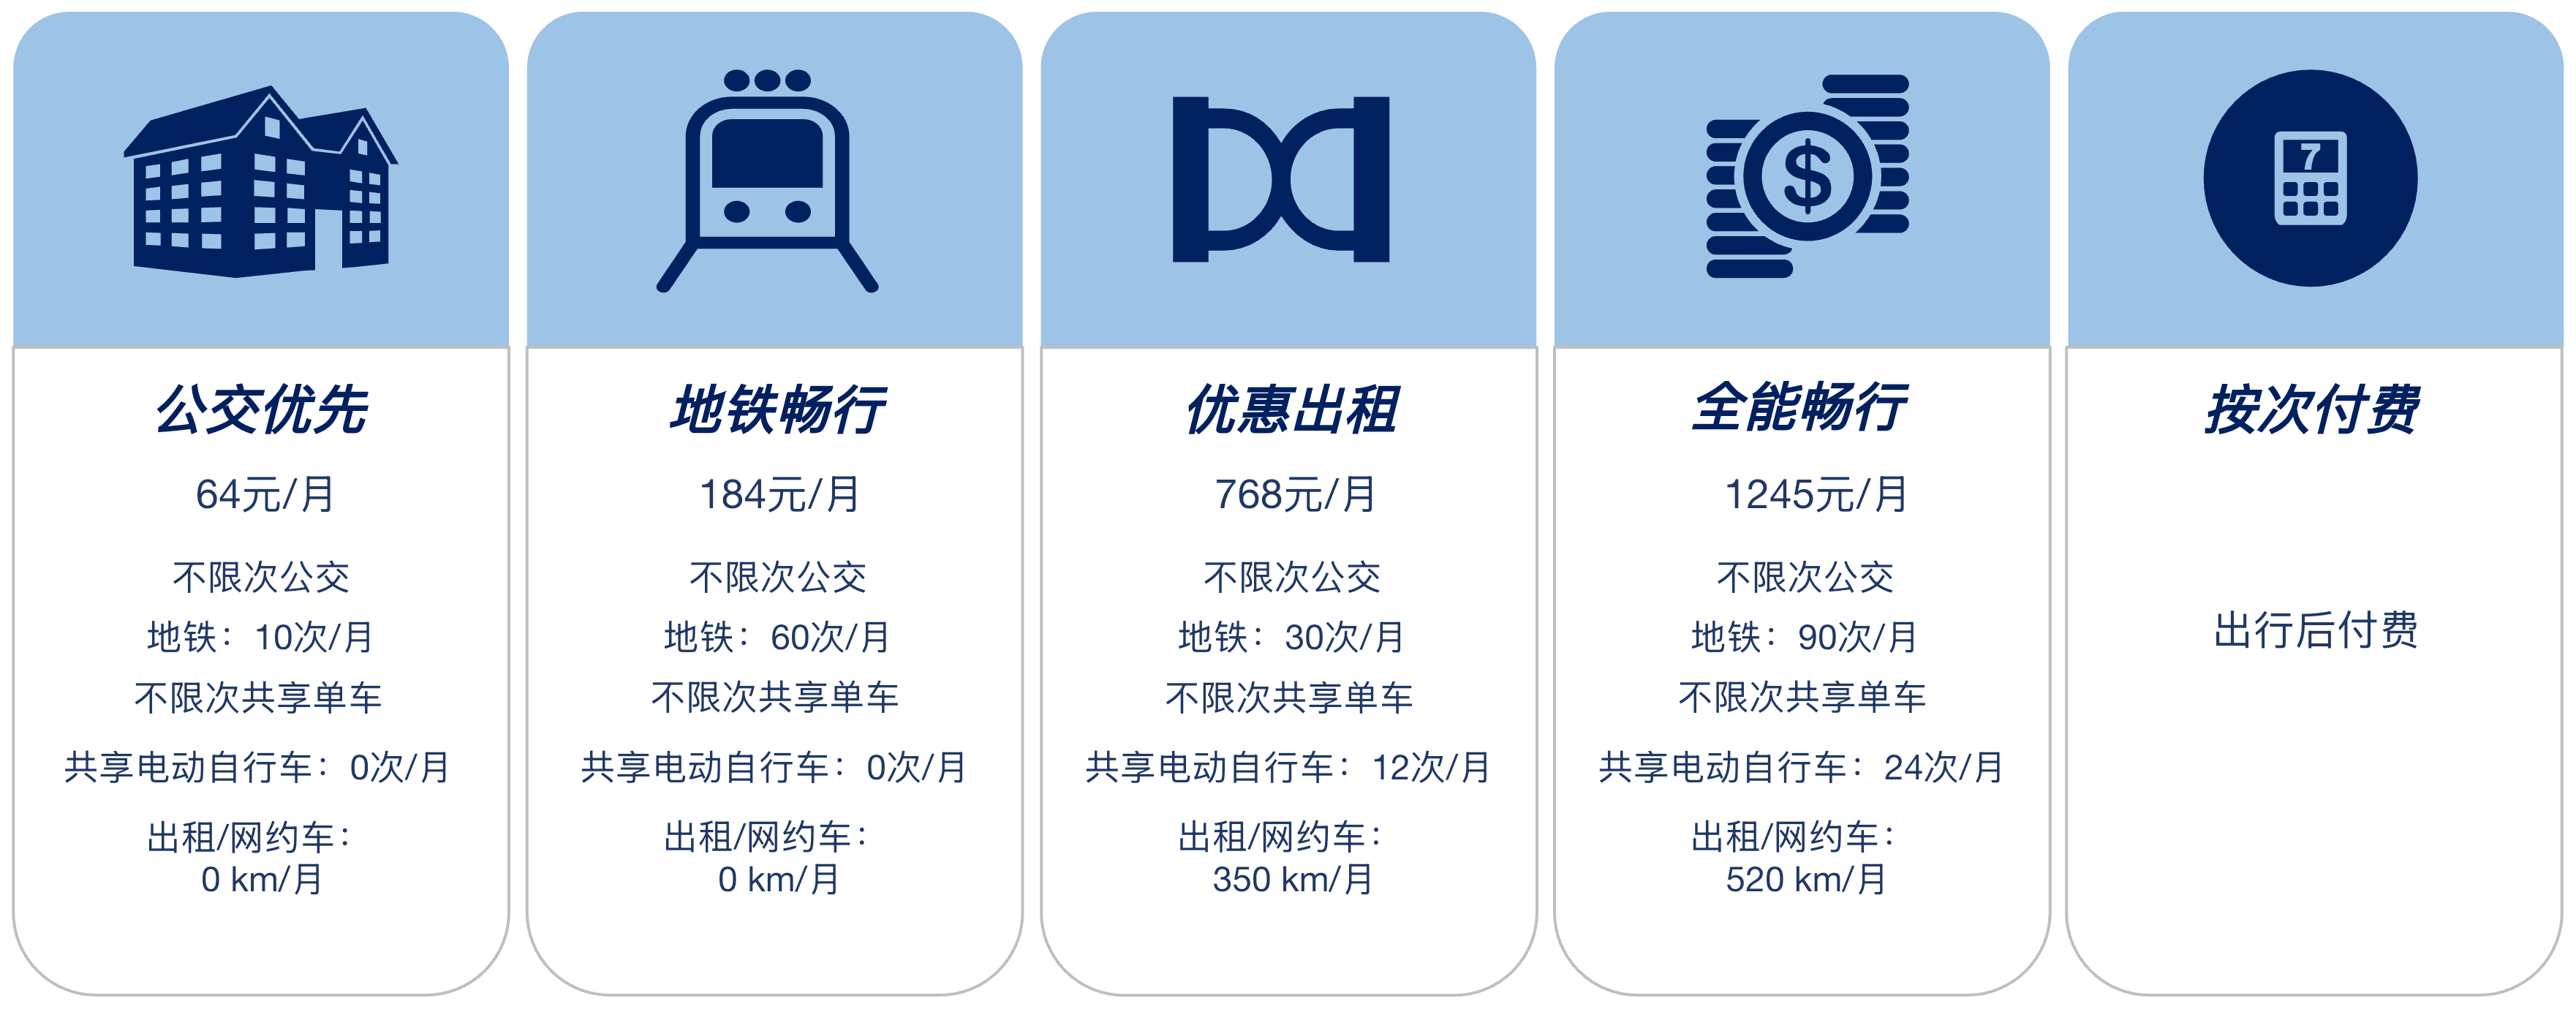
\includegraphics[width=0.92\textwidth]{figures/appendixC/sp_bundle_example.png}
\end{center}
\par\medskip

\noindent\textbf{32．在上述仅限个人使用的订阅服务方案中，您会选择哪一个：}\\
\qbox 公交优先\quad \qbox 地铁畅行\quad \qbox 优惠出租\quad \qbox 全能畅行\quad \qbox 按次付费

\clearpage
\vspace{0.6em}
\noindent\textbf{第四部分\quad 出行态度调查}

请选择您对以下各项表述的赞同程度，其中数字1$\sim$5依次表示由``非常不赞同''到``非常赞同''。

\par\medskip
{\small
\setlength{\tabcolsep}{6pt}
\begin{longtable}{>{\centering\arraybackslash}m{1.1cm}>{\raggedright\arraybackslash}m{7.4cm}>{\centering\arraybackslash}m{4.6cm}}
\toprule
序号 & 问题表述 & 非常不赞同~1$\sim$5~非常赞同\\
\midrule
\endfirsthead
\multicolumn{3}{l}{\small（续表）}\\
\toprule
序号 & 问题表述 & 非常不赞同~1$\sim$5~非常赞同\\
\midrule
\endhead
\midrule
\multicolumn{3}{r}{\small 续下页}\\
\endfoot
\bottomrule
\endlastfoot
1 & 出行便捷对我很重要 & \qbox1\ \qbox2\ \qbox3\ \qbox4\ \qbox5 \\
2 & 出行经济对我很重要 & \qbox1\ \qbox2\ \qbox3\ \qbox4\ \qbox5 \\
3 & 出行舒适对我很重要 & \qbox1\ \qbox2\ \qbox3\ \qbox4\ \qbox5 \\
4 & 出行可靠对我很重要 & \qbox1\ \qbox2\ \qbox3\ \qbox4\ \qbox5 \\
5 & 我偏好等待时间更短的出行 & \qbox1\ \qbox2\ \qbox3\ \qbox4\ \qbox5 \\
6 & 我偏好出行时间更短的出行 & \qbox1\ \qbox2\ \qbox3\ \qbox4\ \qbox5 \\
7 & 我乐于享受出行优惠 & \qbox1\ \qbox2\ \qbox3\ \qbox4\ \qbox5 \\
8 & 我愿意尝试新鲜事物 & \qbox1\ \qbox2\ \qbox3\ \qbox4\ \qbox5 \\
9 & 我希望在单一平台上规划出行 & \qbox1\ \qbox2\ \qbox3\ \qbox4\ \qbox5 \\
10 & 我认为新型出行方式会提升我的出行品质 & \qbox1\ \qbox2\ \qbox3\ \qbox4\ \qbox5 \\
11 & 我认为MaaS能让我的出行更高效 & \qbox1\ \qbox2\ \qbox3\ \qbox4\ \qbox5 \\
12 & 我认为MaaS能降低我的出行成本 & \qbox1\ \qbox2\ \qbox3\ \qbox4\ \qbox5 \\
13 & 我不希望我的出行计划被打乱 & \qbox1\ \qbox2\ \qbox3\ \qbox4\ \qbox5 \\
14 & 我认为做计划很重要 & \qbox1\ \qbox2\ \qbox3\ \qbox4\ \qbox5 \\
15 & 以低碳方式出行对我很重要 & \qbox1\ \qbox2\ \qbox3\ \qbox4\ \qbox5 \\
16 & 以环保方式出行对我很重要 & \qbox1\ \qbox2\ \qbox3\ \qbox4\ \qbox5 \\
17 & 在线出行规划可能侵犯我的隐私 & \qbox1\ \qbox2\ \qbox3\ \qbox4\ \qbox5 \\
18 & 目前可获得的出行信息不够充分 & \qbox1\ \qbox2\ \qbox3\ \qbox4\ \qbox5 \\
19 & 我对出行的安全性感到满意 & \qbox1\ \qbox2\ \qbox3\ \qbox4\ \qbox5 \\
20 & 我认为当前的共享出行性价比高 & \qbox1\ \qbox2\ \qbox3\ \qbox4\ \qbox5 \\
21 & 目前获得的出行信息是准确的 & \qbox1\ \qbox2\ \qbox3\ \qbox4\ \qbox5 \\
22 & 我愿意用手机提前规划出行 & \qbox1\ \qbox2\ \qbox3\ \qbox4\ \qbox5 \\
23 & 出行安全对我很重要 & \qbox1\ \qbox2\ \qbox3\ \qbox4\ \qbox5 \\
24 & 我认为开车出行更舒适 & \qbox1\ \qbox2\ \qbox3\ \qbox4\ \qbox5 \\
25 & 我不愿改变惯常的出行方式 & \qbox1\ \qbox2\ \qbox3\ \qbox4\ \qbox5 \\
\end{longtable}
}

\indent
\zihao{5}
